\documentclass[crop,tikz]{standalone}
\usetikzlibrary{backgrounds}
\colorlet{blue}{cyan}
\tikzset{
  inverted/.style = {
    color=white,
    background rectangle/.style={fill},
    show background rectangle
  }
}

\usepackage{pgfplots}
\pgfplotsset{compat=1.16}
\tikzset{>=latex}

\colorlet{green}{green}

\pgfplotsset{
  inverted/.style = {
    every axis legend/.append style={
      draw=white,
      fill=white,
      text=white
    }
  },
  every non boxed x axis/.append style={
    axis line style={-latex}
  },
  every non boxed y axis/.append style={
    axis line style={-latex}
  },
  every non boxed z axis/.append style={
    axis line style={-latex}
  },
}

\begin{document}
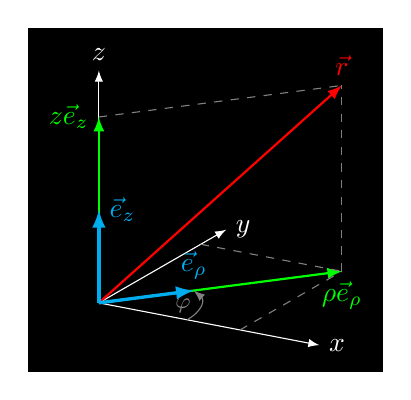
\begin{tikzpicture}[inverted,inverted]
  \pgfmathsetmacro{\px}{1.6};
  \pgfmathsetmacro{\py}{2};
  \pgfmathsetmacro{\pz}{2};
  \begin{axis}[inverted,
    width=6cm,
    height=6cm,
    view={30}{20},
    xlabel={$x$},
    ylabel={$y$},
    zlabel={$z$},
    xmin=0,xmax=2.5,
    ymin=0,ymax=2.5,
    zmin=0, zmax=2.5,
    xtick=\empty,
    ytick=\empty,
    ztick=\empty,
    axis x line=middle,
    axis y line=middle,
    axis z line=middle,
    xlabel style={right},
    ylabel style={right},
    zlabel style={above},
    clip=false,
    ]
    % vector to space point
    \draw[->,red,thick]  (axis cs:0,0,0) -- (axis cs: {\px},{\py},{\pz}) node[above] { $\vec{r}$ };
    % projections onto x-y-plane and z-axis
    \draw[->,green,thick] (axis cs:0,0,0) -- (axis cs: {\px},{\py},0) node[below] { $\rho\vec{e}_\rho$ };
    \draw[->,green,thick] (axis cs:0,0,0) -- (axis cs: 0,0,{\pz}) node[left] { $z\vec{e}_z$ };
    % help lines for projections
    \draw[gray,dashed] (axis cs:{\px},{\py},0) -- (axis cs: {\px},{\py},{\pz});
    \draw[gray,dashed] (axis cs:0,0,{\pz}) -- (axis cs: {\px},{\py},{\pz});
    \draw[gray,dashed] (axis cs:{\px},0,0) -- (axis cs: {\px},{\py},0);
    \draw[gray,dashed] (axis cs:0,{\py},0) -- (axis cs: {\px},{\py},0);
    % unit vectors
    \draw[->,blue,very thick] (axis cs:0,0,0) -- (axis cs: 0,0,1) node[right] { $\vec{e}_z$ };
    \draw[->,blue,very thick] (axis cs:0,0,0) -- (axis cs: {\px/sqrt(\px^2 + \py^2)},{\py/sqrt(\px^2 + \py^2)},0) node[above] { $\vec{e}_\rho$ };
    % polar angle
    \draw[->,gray] (axis cs:1,0,0) arc (0:{atan(\py/\px)}:1) node[left,pos=0.5] {\footnotesize $\varphi$};
  \end{axis}
\end{tikzpicture}
\end{document}
